\part{Teoria}

\chapter{Mobile Computing}
\label{mobile-computing}

Negli ultimi anni il numero di dispositivi connessi ad Internet è
aumentato molto velocemente, tant'è che per il 2020 ci si aspetta di
avere 50 miliardi di dispositivi connessi, per lo più mobile, anche se
per il PC resta tra gli strumenti preferiti per il mondo del lavoro.

Il termine \textbf{Mobile Computing} ha molto definizioni, che possono
essere racchiuse in ``\emph{Si parla di \textbf{Mobile Computing} quando
un processo di lavoro che prima veniva effettuato per forza in una
posizione fissa viene spostato in una posizione più dinamica}'', ovvero
racchiude tutte le tecnologie che permettono alle persone di accedere a
dei servizi \textbf{ovunque,} in qualsiasi modo e in qualsiasi momento.

Spostarsi in ambito mobile ha vari vantaggi:

\begin{itemize}
\item
  \begin{quote}
  ci si può connettere ovunque e in ogni momento
  \end{quote}
\item
  \begin{quote}
  con le tecnologie Wireless si possono portare le telecomunicazioni in
  ogni luogo senza bisogno di infrastruttura
  \end{quote}
\item
  \begin{quote}
  nuove possibili applicazioni
  \end{quote}
\end{itemize}

Ma il mobile può essere visto sotto un punto di vista fisico, con il
device che si sposta nello spazio, o da un punto di vista logico, con il
software eseguito nel cloud.

Il bello di questo ambito è che racchiude varie branche dell'ingegneria
e pertanto viene spinto da vari fattori:

\begin{itemize}
\item
  \begin{quote}
  \textbf{Miniaturizzazione}: device sempre più piccoli
  \end{quote}
\item
  \begin{quote}
  \textbf{Connettività}: Wireless sempre più diffuso e performante
  (4G-LTE, Bluetooth, WiFi)
  \end{quote}
\item
  \begin{quote}
  \textbf{Portabilità}: device più piccoli sono più facili da
  trasportare
  \end{quote}
\item
  \begin{quote}
  \textbf{Convergenza}: lo stesso dispositivo racchiude le funzionalità
  di più dispositivi
  \end{quote}
\item
  \begin{quote}
  \textbf{Divergenza:} creazione di dispositivi altamente specializzati
  \end{quote}
\item
  \begin{quote}
  \textbf{App e Ecosistemi digitali}: tecnologie e applicazioni che
  interagiscono tra di loro
  \end{quote}
\end{itemize}

Le principali sfide sono:

\begin{itemize}
\item
  \begin{quote}
  \textbf{Vincoli sulle risorse}: sono utilizzate delle batterie e il
  consumo energetico è elevato (CPU, schermo, antenne, sensori, ecc.) e
  la memoria è limitata
  \end{quote}
\item
  \begin{quote}
  \textbf{Connettività mobile}: varie tipologie con prestazioni diverse,
  interferenze
  \end{quote}
\item
  \begin{quote}
  \textbf{Sicurezza}: le comunicazioni Wireless sono più facili da
  intercettare, furti dei dispositivi mobile
  \end{quote}
\end{itemize}

\section{Ubiquitous Computing }\label{ubiquitous-computing}

la tecnologia più avanzata è quella che tende a sparire, computer sempre
più piccoli, UI sempre più grand (VR, AR). Esempio del Xerox
Parc
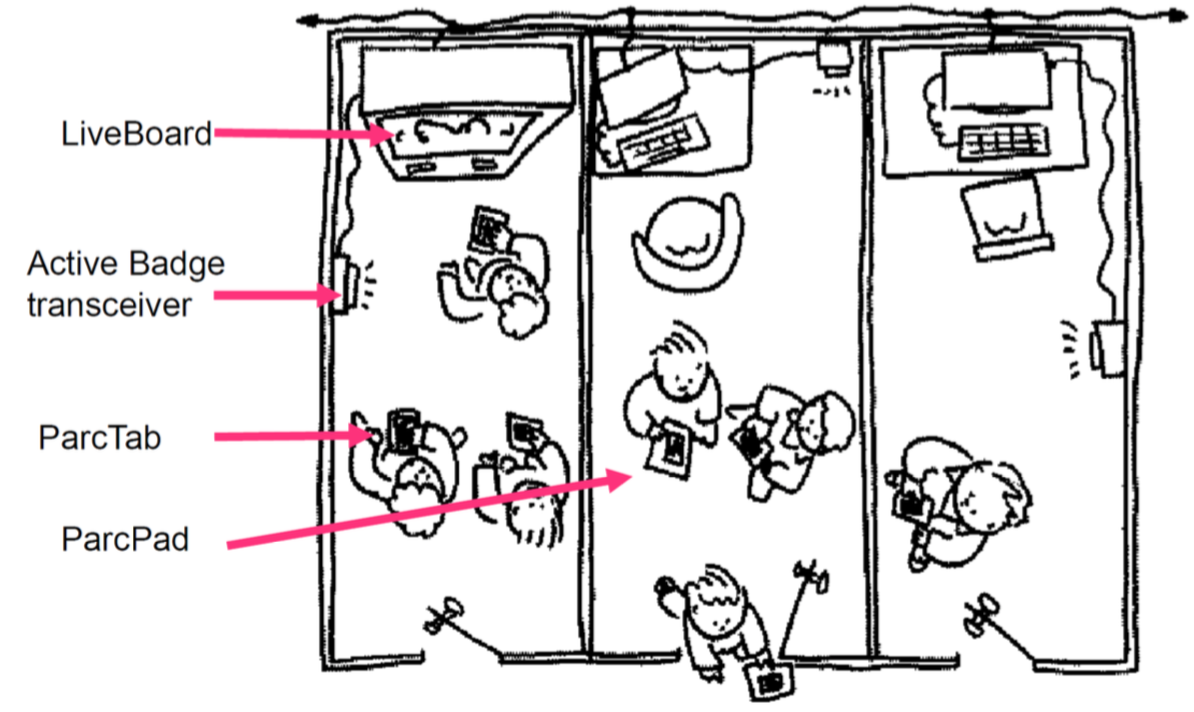
\includegraphics[width=2.97237in,height=1.77256in]{image5.png}
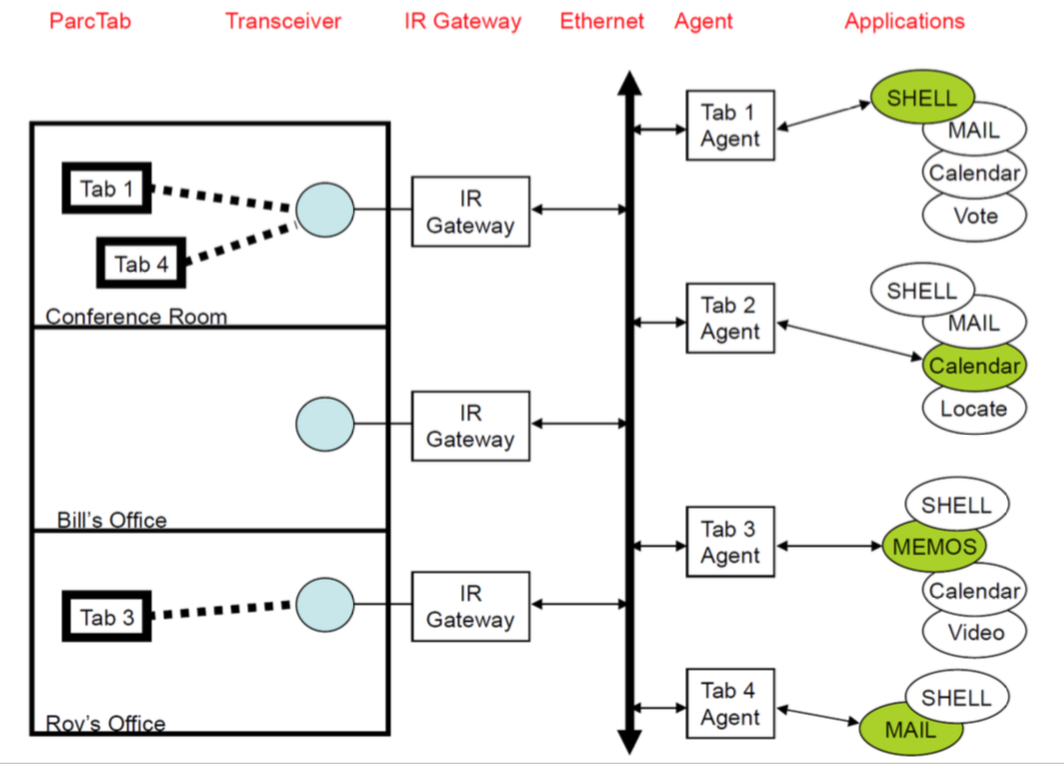
\includegraphics[width=2.82457in,height=2.02693in]{image6.png}

Siamo quindi alla terza era del \textbf{comuputing:}

\begin{itemize}
\item
  \begin{quote}
  Era 1: Mainframe computing, tanti utenti per un singolo computer
  \end{quote}
\item
  \begin{quote}
  Era 2: Personal computing, un utente per ogni computer
  \end{quote}
\item
  \begin{quote}
  Era 3: Ubiquitous computing, un utente per tanti computer.
  \end{quote}
\end{itemize}

Da notare che in questa terza era non tutti i computer sono dell'utente
(smartphone, PC, ecc.) ma alcuni vengono incontrati spostandosi e
sfruttati opportunisticamente, come camere di sorveglianza, sensori,
chioschi per le informazioni, la cosa fondamentale è che tutti questi
computer siano tra loro \textbf{connessi} e \textbf{programmabili}.
Questo perché già da tempo ci sono computer in ogni dove, ma questi non
sono tra loro connessi.

Si va quindi a coprire sia i computer special purpose che quelli general
purpose, con una varietà di dispositivi enormi,

\textbf{Ubiquitous computing} è quindi una nuova era in cui le persono
sono circondate da molti computer connessi tra loro che collaborano in
modo spontaneo e che possono essere:

\begin{itemize}
\item
  \begin{quote}
  indossati o trasportati
  \end{quote}
\item
  \begin{quote}
  incontrati in vari luoghi
  \end{quote}
\item
  \begin{quote}
  parte di oggetti fisici
  \end{quote}
\end{itemize}

ma tutti intuitivi da utilizzare e difficili da notare.

Alcune tipologie di dispositivi sono:

\begin{itemize}
\item
  \begin{quote}
  \textbf{Sensors networks} piccoli computer dotati di sensori che
  raccolgono le informazioni sull'ambiente circostante
  \end{quote}
\item
  \begin{quote}
  \textbf{Wearables}
  \end{quote}
\item
  \begin{quote}
  \textbf{Networked appliances} come i distributori automatici che
  segnalano informazioni sul loro stato
  \end{quote}
\item
  \begin{quote}
  \textbf{Smart labels} come RFID o beacon bluetooth
  \end{quote}
\end{itemize}

C'è quindi un esplosione esponenziale di dispositivi connessi ad
internet che comunicano tra loro senza che l'intervento dell'utente e
quindi la scalabilità del sistema diventa l'aspetto principale.

Ci sono quindi molte nuove sfide che derivano dalla presenza di tutti
questi dispositivi che riguardano la protezione dei dati, l'affidabilità
dei dispositivi e delle comunicazioni, la diversità e l'intrusione che
deve essere limitata per evitare di distrarre l'utente.

L'interazione con l'utente è particolarmente problematica perché deve
essere \textbf{context aware} ovvero il software deve adattarsi al
contesto in cui viene utilizzato (in macchina, in corsa, ecc) e deve
poter essere utilizzato in \textbf{varie modalità} ovvero deve
supportare più modalità di input/output in modo da potersi adattare
meglio al contesto.

\section{S.C.A.L.E.}\label{s.c.a.l.e.}

Le sfide principali (\textbf{integrazione dei sistemi} e \textbf{humane
computing}) possono essere organizzate secondo la tassonomia SCALE:

\begin{itemize}
\item
  \begin{quote}
  \textbf{Scalability} come supportare miliardi di dispositivi connessi
  in tutto il mondo? Quindi sia a livello di connettività che di
  capacità di calcolo e integrazioni
  \end{quote}
\item
  \begin{quote}
  \textbf{Connectivity} come connettere tutti questi dispositivi con le
  reti wireless? Utilizzo di comunicazione ad eventi ccn il paradigma
  \textbf{push} e con la cooperazione tra i dispositivi, creando delle
  reti stratificate \textbf{P2P,} opportunistiche (ad-hoc) e allocando
  dinamicamente le risorse secondo una filosofia cloud.
  \end{quote}
\item
  \begin{quote}
  \textbf{Adaptability} come adattare questo al contesto d'uso? Utilizzo
  dei sensori per capire il contesto, ma anche attraverso dei modelli
  predeterminati o inferendo in contesto da altre informazioni. Ma anche
  a livello utente, in base alle sue esperienze, necessità e preferenze.
  \end{quote}
\item
  \begin{quote}
  \textbf{Liability (security)} come garantire la sicurezza? Non c'è più
  un sistema centralizzato e nella comunicazione machine-to-machine non
  è più utilizzabile il sistema di certificati, perché non si può sempre
  avere un'autorità centrale, quindi non si può fare crittografia
  end-to-end.
  \end{quote}
\item
  \begin{quote}
  \textbf{Ease-of-use} i vari sistemi devono essere facili ed intuitivi
  da utilizzare con più modalità di input (es: movimento degli occhi,
  controlli vocali, feedback audio, ecc.)
  \end{quote}
\end{itemize}

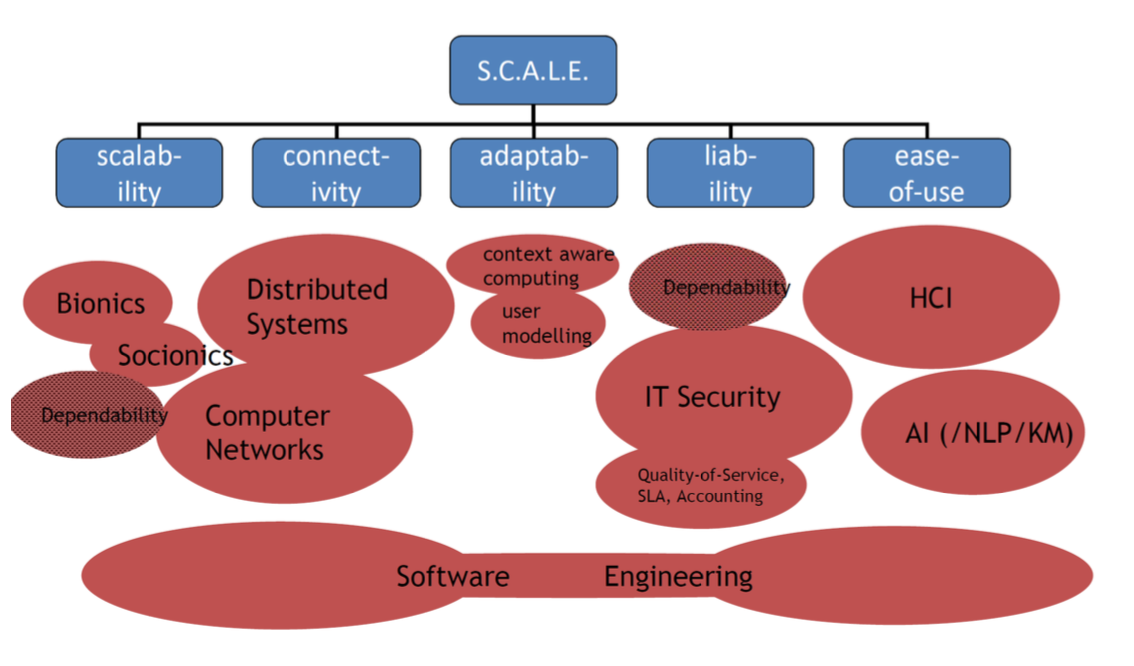
\includegraphics[width=3.44704in,height=2.02127in]{image3.png}

\section{Use cases/Must know}\label{use-casesmust-know}

\textbf{Internet of Things} è il termine principalmente utilizzato dalla
stampa per parlare di ubiquitous computing.

\textbf{AutoID} standard per la definizione di etichette identificative
tramite RFID inizialmente sviluppato al MIT.

\textbf{OSGi} standard per la distribuzione/revisione di codice o
servizi attraverso internet per i sistemi embedded/smart.

\textbf{Edge Network} \textbf{Integration} sistema di reti ponte che
permettono di collegare reti esistenti ma basate su stack diversi (???)

\textbf{Smart home} insieme di progetti per la creazione di una casa
intelligente, inserendo attuatori e sensori nei vari oggetti per
automatizzare/risparmiare energia. Sembra più probabile
l'implementazione solo in ambito business perché ci sono investimenti
maggiori

\textbf{Smart item} dispositivi con risorse limitate specifici per
determinate applicazioni.

\textbf{LAURA} sistema di localizzazione/monitoraggio dei pazienti nelle
strutture sanitarie.

\textbf{DrivingStyles} progetto che studia la correlazione tra il
comportamento dell'utente nel traffico e il suo battito cardiaco.

\textbf{SmarParking} occupazione e prenotazione dei parcheggi mediante
app.

\textbf{WaterBot} monitoraggio dei consumi di acqua in casa con aspetti
di gamification per incentivare il risparmio.
